% !TeX document-id = {55487e37-df6e-4d5b-af2f-b0275db5df41}
%%
%% This is file `sample-manuscript.tex',
%% generated with the docstrip utility.
%%
%% The original source files were:
%%
%% samples.dtx  (with options: `manuscript')
%% 
%% IMPORTANT NOTICE:
%% 
%% For the copyright see the source file.
%% 
%% Any modified versions of this file must be renamed
%% with new filenames distinct from sample-manuscript.tex.
%% 
%% For distribution of the original source see the terms
%% for copying and modification in the file samples.dtx.
%% 
%% This generated file may be distributed as long as the
%% original source files, as listed above, are part of the
%% same distribution. (The sources need not necessarily be
%% in the same archive or directory.)
%%
%% The first command in your LaTeX source must be the \documentclass command.
%%%% Small single column format, used for CIE, CSUR, DTRAP, JACM, JDIQ, JEA, JERIC, JETC, PACMCGIT, TAAS, TACCESS, TACO, TALG, TALLIP (formerly TALIP), TCPS, TDSCI, TEAC, TECS, TELO, THRI, TIIS, TIOT, TISSEC, TIST, TKDD, TMIS, TOCE, TOCHI, TOCL, TOCS, TOCT, TODAES, TODS, TOIS, TOIT, TOMACS, TOMM (formerly TOMCCAP), TOMPECS, TOMS, TOPC, TOPLAS, TOPS, TOS, TOSEM, TOSN, TQC, TRETS, TSAS, TSC, TSLP, TWEB.
% \documentclass[acmsmall]{acmart}

%%%% Large single column format, used for IMWUT, JOCCH, PACMPL, POMACS, TAP, PACMHCI
\documentclass[acmlarge,screen]{acmart}
% !TeX TXS-program:compile = txs:///pdflatex/[--shell-escape]

%%%% Large double column format, used for TOG
%\documentclass[acmtog, authorversion]{acmart}

%%%% Generic manuscript mode


%%
%% \BibTeX command to typeset BibTeX logo in the docs
\AtBeginDocument{%
  \providecommand\BibTeX{{%
    \normalfont B\kern-0.5em{\scshape i\kern-0.25em b}\kern-0.8em\TeX}}}

\usepackage{listings}
\usepackage{minted} 
\usepackage{subcaption}
\usepackage{float}
\usepackage{wrapfig}
\restylefloat{figure}
\usemintedstyle{friendly}
\graphicspath{ {../images/} }



%%
%% The majority of ACM publications use numbered citations and
%% references.  The command \citestyle{authoryear} switches to the
%% "author year" style.
%%
%% If you are preparing content for an event
%% sponsored by ACM SIGGRAPH, you must use the "author year" style of
%% citations and references.
%% Uncommenting
%% the next command will enable that style.
%%\citestyle{acmauthoryear}

%%
%% end of the preamble, start of the body of the document source.
\begin{document}

%%
%% The "title" command has an optional parameter,
%% allowing the author to define a "short title" to be used in page headers.
\title{UVU MCS Graduate Paper}

%%
%% The "author" command and its associated commands are used to define
%% the authors and their affiliations.
%% Of note is the shared affiliation of the first two authors, and the
%% "authornote" and "authornotemark" commands
%% used to denote shared contribution to the research.

\author{Benjamin Stoneking}
\affiliation{%
 \institution{Candidate}
}
\email{benjamin.stoneking@protonmail.com}

\author{Frank Jones}
\affiliation{%
 \institution{Advisor}
}
\email{frankj@uvu.edu} 

%%
%% By default, the full list of authors will be used in the page
%% headers. Often, this list is too long, and will overlap
%% other information printed in the page headers. This command allows
%% the author to define a more concise list
%% of authors' names for this purpose.
\renewcommand{\shortauthors}{Candidate First Last}

%%
%% The abstract is a short summary of the work to be presented in the
%% article.
\begin{abstract}
	The project explores the implementation of an embedded real-time digital audio synthesizer. Emphasis is placed on leveraging the inherent strengths of the hardware (timers, hardware interrupts, etc) to produce a reliable musical instrument. The project is a focused exercise in implementing a digital audio processing pipeline with software implementations of common components such as oscillators, pitch control, signal gain attenuation, and filtering. It illustrates the process of implementing a capable, complex and extendable embedded system on a platform with limited processing power. The final product is a fundamental subtractive synthesizer: It responds to input from generic MIDI devices to produce an audio signal. It applies volume dynamics and timbre control to the signal using envelopes and filters. The device has a hardware interface consisting of knobs, encoders, and a screen allowing direct, real-time manipulation of the processing. A PC application can control the system remotely. The system is robust and extensible. Numerous features can be added. The project code base was written to be efficient in its size and speed. The project firmware source is about 2,000 lines with with PC application and test code bringing it up to 2,500.
\end{abstract}

%%
%% Keywords. The author(s) should pick words that accurately describe
%% the work being presented. Separate the keywords with commas.
\keywords{digital, audio, synthesis, embedded, microcontroller, real-time, midi, hardware, oscillator, filter, envelope, DSP, prototype, discrete-time, continuous-time, analog}

%%
%% This command processes the author and affiliation and title
%% information and builds the first part of the formatted document.
\maketitle

\section{Introduction}
\subsection{Purpose}
	The acquisition of musical gear is a common obsession of musicians around the world. The cost of gear for performance or music production presents a major financial struggle to those already working with a tight budget. A common thought occurs: "What if I just make my own X? Maybe I can save some money." This discussion occurs frequently within online and offline discourse. Often, musicians who have experience making their own digital or analog instruments give the same answer: "Yes. You can just make your own X. But no. You won't save any money. You will end up spending more and you should just save up some cash to just buy your gear." I've walked this path myself and found this conclusion to be true but with a small caveat: You can in fact save money by making your audio production tool as a \textbf{digital system}. You can write as much software as you want. You can refactor and rebuild you software tool over and over, and never spend a dime. When physical electronic components are removed from the equation, you can make all your music production gear for free. This caveat has a caveat of its own: This takes substantial time. Time is money. Therefore, every hour spent in implementing your system is implicitly adding to the hypothetical price tag of your system.
	
	Of course, implementing your own digital audio processing tools can be seen as reinventing the wheel. This project can be characterized as \textit{yet another} software synthesizer. The purpose of this project is not to create a product that is competitive with the mainstream market, but to discover the process and patterns of building an audio synthesis system on an embedded platform. My education has had me walk through the process of making \textit{yet another} database management system, and \textit{yet another} virtual machine. Unsurprisingly, my database hasn't replaced MySQL and my virtual machine has not replaced the Java Virtual Machine. Reinventing the proverbial wheel does not make the effort fruitless. Valuable wisdom and knowledge of how complex systems work is gained on the journey to replicate existing solutions. I applied this same principle to my master's project: Make \textit{yet another} digital synthesizer on an embedded microcontroller. \textbf{The endgame of this project is the journey itself}:
	\begin{itemize}
		\item Learn how to implement a complex real-time embedded system
		\item Develop a modular digital audio pipeline
		\item Build a hardware interface to control the system
		\item Discover what invaluable knowledge can be extracted from the experience
	\end{itemize}
	
\subsection{Concepts}
	To help the reader get up to speed, following is a short list of recurring words and their definitions as they relate to audio synthesis and this project.
	\begin{itemize}
		\item \textbf{Oscillator:} Generally speaking, an oscillator is a function generator. Generates a repeating signal at a specified frequency much like the function generator of an oscilloscope. The starting point of the audio signal chain.
		\item \textbf{Monophonic:} A synth that can play only one pitch at a time.
		\item \textbf{Polyphonic:} A synth that can play two or more discrete notes at a time.
		\item \textbf{Voice:} A structure containing one or more oscillators. One voice can play one pitch at a time. Voices are used to support polyphony.
		\item \textbf{Modulation:} The usage of an analog or digital signal as a function to alter the inputs of another function.
		\item \textbf{Envelope:} A multiphase linear signal generator. Used as a modulation source for other signals.
		\item \textbf{Low Frequency Oscillator (LFO):} An oscillator producing signals below human hearing. Used as a modulation source.
		\item \textbf{Low Pass Filter:} A filter that removes high frequencies from a signal past a certain cutoff point.
		\item \textbf{High Pass Filter:} Like a low pass filter but removing low frequencies.
		\item \textbf{Sample Rate:} Refers to how often a digital signal is being sampled in samples per second.
		\item \textbf{Bit Depth:} How many bits are used to represent a digital sample.
		\item \textbf{Digital to Analog Converter (DAC):} A hardware component used to output a digital signal as an analog voltage signal.
		\item \textbf{MIDI:} Musical Instrument Data Interface. A communications protocol for controlling electronic instruments, computer software, lighting systems etc. Supports hundreds of different kinds of messages. "Note On" and "Note Off" messages are the most common and contain pitch and velocity (how loudly the note is being played).
	\end{itemize}

\subsection{Project Criteria}
	\paragraph{The aim of this project was to accomplish the task of creating this device, document the architecture, process and the lessons learned.}What is a valid working architecture to making such a system? Where does one begin? What kind of failure and setbacks should be expected? Can it be done within a reasonable amount of time without substantial reliance on previously existing frameworks and libraries? What sort of mathematical and technical knowledge is required?
	\subsubsection{Minimum Requirements}
	\label{requirements}
	This implementation of a subtractive synthesizer must meet the following minimum requirements (see Concepts for definitions):
	\begin{enumerate}
		\item Produce audio at a minimum quality of 44.1khz and 16 bit-depth (Industry standard quality)
		\item Be compatible with any generic MIDI keyboard.
		\item \textbf{Oscillator} module must generate the most common wave forms: Sin, sawtooth, square, triangle and white noise
		\item Support polyphony, with capability to play up to eight discrete notes at a time.
		\item Support mixing of multiple oscillators to generate hybrid waveforms.
		\item Support \textbf{envelope} signal generation for dynamic modulation of other signals.
		\item Implement a \textbf{Filter} module that supports lowpass, highpass and bandpass filtering, able to adjust frequency cutoff and resonance in real-time.
		\item Implement \textbf{low-frequency oscillator (LFO)} module configurable to modulate the signals of other modules within the system.
		\item Provide a memory bank where users can save their "patches" to use later.
		\item Provide interaction between the user and the system via a \textbf{hardware interface}. User inputs include a MIDI jack for keyboard input and knobs for navigating a menu and changing parameters. Outputs include a 1/8" audio output jack for playback with headphones and speakers and a menu screen for communicating the system state to the user. Knobs adapt to the context of the menu to appropriately adjust parameters.
	\end{enumerate}
	
	\subsubsection{Constraints}
	In order to maximize the learning potential of this project and focus on the process rather than the final destination, I set a few restrictions:
	\begin{enumerate}
		\item Language: Implement the firmware in a low-level programming language such as C/C++. Complex, non-static data structures should be avoided to keep the system efficient, transparent and stable.
		\item Libraries: Utilize only the standard C/C++ libraries with the exception of a Hardware Abstraction Layer to minimize hardware peripheral set up time. 
		\item References: Put forth every effort to learn the mathematical concepts of DSP and implement them without referencing existing solutions.
	\end{enumerate}
	
\subsection{Results}
	\subsubsection{What did I learn?}
	
	\paragraph{Choose your device platform carefully} I chose the audio development board Daisy by Electro-Smith. It is marketed as an attractive option for musicians to implement their dream systems because of its high resolution digital to analog (DAC) converter and painless hardware peripheral abstractions. It turned out to not be as mature and stable as I hoped and had many issues with drivers, pin connections and lacking support for certain interrupt service routines. Initially, it was difficult to see that Daisy may not have been the best option for implementing a system scoped beyond a hobbyist project. The platform was designed for musicians to implement simpler systems with highly abstracted development libraries and programming languages/frameworks like MaxMSP, Puredata and Arduino. More attention and care appears to have been put into supporting these tools and making them work well while some lower level capabilities were sidelined.
	
	\paragraph{Prototype hardware incrementally} After spending several months setting up my hardware peripherals on a breadboard and implementing core functionality, I felt the need to migrate the system off a breadboard to a more permanent and stable fixture. It was at this point I learned the cost of trying to do too much at once. I tried to design a soldered circuit board able to be embedded in an enclosure that was yet to be designed. My thought was that it may take several revisions of the enclosure before I knew where all my knobs, encoders, inputs, outputs and screen needed to be for ease of use and optimal functionality. I built up flying wire harnesses for all peripherals so that they could be moved around to test out different enclosure layouts. The result was an absolute mess of wires that were susceptible to interference. My first step in taking the system off the breadboard should have been simply solder my components into logical sections on perf board and make the system work as it did on the breadboard. It would not have been an optimal design and I would have had to do another revision to get the system installed in an enclosure. But I would have saved so much time soldering and troubleshooting a sloppy design that ultimately failed. Such time could have been allocated to adding additional capabilities to the software.
	
	\paragraph{Decouple pure software functions from hardware and test independently} My workflow for the entirety of the project was \textbf{write code, compile, flash, test, repeat}. This involves a lot of waiting. Waiting for the compiler. Waiting for the bootloader. Waiting for the flash process to complete. If I wrote my code more carefully to not be so tightly coupled to the Daisy system, I could have written some pure software test fixture code that runs on my host PC to test my different synth components independently. This would have facilitated a much tighter development and testing loop. In addition, the modules would be more portable and easy to integrate into other systems.
	
	\paragraph{Purchase hardware components from trusted sources and verify functionality} I made the mistake of sourcing some components from Amazon. The cheap price and quick delivery was too much of a temptation. I ended up wasting several agonizing days troubleshooting and debugging software all because of one encoder in a bag of ten. The factory happened to solder its PCB in reverse and it was completely defective. I assumed my code was the problem. Only after hooking the offending part up to a multimeter was I able to see the problem. I replaced the part and my system worked without a single change to the software. While it is reasonable to suspect your implementation may be flawed before blaming hardware, manufactured parts should be trusted, but also verified.
	
	\subsubsection{Complexity}
	\paragraph{Looking at the code does not always accurately express the effort and time invested to develop a solution}. Writing driver code for the project was a long process. It required reading long data sheets for devices and to learn how they work. Each component required a surprisingly deep level of knowledge to properly communicate with them. Actually writing the code to communicate in the devices specific protocol can be a long process of trial and error. 
	
	\paragraph{Implementing the driver code to communicate with the LCD screen over I2C took a significant amount of time} Many hours were spent writing low level functions to pack a lot of information into just several bytes of data that perform one function. These functions need to be written to perform a seemingly insignificant task like writing a single character to the screen, moving the cursor, erasing the screen or just configure the screen. Additional functions need to be written using these new driver level functions to do things like write a complete string to a specific line or create a menu scrolling effect. After all this time is spent implementing these necessary functions, the driver code may only be one or two hundred lines long. This experience demonstrated to me the fact that lines of code is not always an accurate model for determining the complexity of a system.
	
	\subsubsection{Design decisions}
	\paragraph{The final architecture of the system is a hybrid of several architectural patterns}. The system is a \textbf{pipeline architecture}. Synth modules are chained together in a mostly linear fashion. Oscillators generate audio sample data. Samples from multiple oscillators are attenuated and combined into a new sample. The aggregated sample is passed through an envelope modulated attenuator. The sample is then passed to a filter. The filtered samples are passed through an audio fx chain where each effect module processes and passes data down to the next. The samples processed by the fx chain are passed through a master volume attenuator and put into the audio DAC's output buffer. The DAC finally converts the digital signal to an analog signal which plays out the physical speakers.
	
	\begin{figure}
		\includegraphics[width=\linewidth]{Synth_Audio_Pipeline}
		\caption{A high level view of the pipeline structure. Some clarification is necessary. Although the keyboard is not part of the audio pipeline, it is included to clarify how pitches are assigned to voices. The voices comprise the beginning of the pipeline. They own two oscillators each which generate the audio samples. Also encapsulated within each voice is an attenuator and envelope which are used to modulate the output gain of each voice. Output samples from the voices are summed and then attenuated. A simplified description of the processing pipeline is as follows:\\\\ Oscillator -$>$ Amp Envelope -$>$ Sample Sum -$>$ Normalize -$>$ Filter -$>$ FX Chain -$>$ Master Gain -$>$ Output Buffer }
	\end{figure}
	
	
	The system is also \textbf{event driven}. On one hand, the audio DAC interrupt drives the audio processing of the synthesizer pipepline. It is responsible for acquiring a sample from the synth and placing it into the DAC's output buffer (note how the DAC functions both as an event driver and as a component in the pipeline). The hardware timer interrupt processes user input. It uses the processed user input to control the various synth components. Because it runs much slower than the DAC, it also drives some synthesizer components like the envelope which generate modulation source signals rather than audio.
	
	At the same time, the system is also \textbf{modular}. Although modularity is a basic expectation of software design, it plays a much bigger role in synthesis itself. It has been a fundamental principle in synthesis since day one. The first synthesizers were a collection of analog circuit boards completely divorced from one another, and they were only connected by series of physical patch cables that could be endlessly rerouted in different permutations. This core principle is implemented into the software. The data structures are independent modules: oscillators, filters, envelopes and LFOs all able to connect to each other similar to how analog synthesizers are connected by patch cables. Some modules are abstract components, aggregating smaller modules to achieve new functionality. Some modules like the envelope do not directly process audio. Instead, they generate signals parallel to the audio pipeline that affect how \textit{other} modules process data.

\section{Software Architecture and Implementation}

\subsection{A High Level View}
	\paragraph{As mentioned previously, the system is an interrupt driven, highly modular, pipeline architecture} A class called synth is a composition of modules that connect to form an digital audio processing pipeline. Two interrupt service routines function as the main operators of this pipeline: A \textbf{hardware timer} interrupt is responsible for capturing user input to control the synths parameters and the notes it plays. An \textbf{audio} interrupt, triggered by the high resolution DAC is responsible for driving the pipeline to generate digital audio samples and load the samples into the DAC's audio out buffer.
	
	There are five key participants involved in the system:
	\begin{enumerate}
		\item The \textbf{user} operating the system with the keyboard keyboard and hardware peripherals
		\item The \textbf{menu system} communicating the system state to the user
		\item The \textbf{synth} generating audio samples for the DAC
		\item The \textbf{timer interrupt} reading hardware inputs to trigger events
		\item The \textbf{audio interrupt} requesting the next sample to write to the audio output DAC.
	\end{enumerate}

%	\begin{figure}[h]
%		\centering
%		\caption{This sequence is the most common event for the runtime of the system. It represents the idle state when the user is not engaged in the system. The process audio callback is continuously requesting samples from the synth, and the synth is just returning a value of zero. The result is silence for the user. \textit{Note: although the timer appears in active, the interrupt is still occuring with no inputs to detect to trigger events.}}
%		\includegraphics[width=.7\linewidth]{no_note_sequence}
%	\end{figure}

	\begin{figure}[H]
		\centering
		\includegraphics[width=.7\linewidth]{play_note_sequence}
		\caption{A sequence diagram of the interaction of the five main actors. The most common scenario is the user playing notes on the keyboard. The timer interrupt detects the MIDI message from the keyboard and triggers a \textit{note on} event for the synth. The synth responds by activating one of its voices and setting the voice's pitch according to the note on event. Next time the audio interrupt occurs, the synth will generate and return an audio sample from that voice. The audio interrupt puts the sample into the DAC buffer which plays out the speakers for the user. Audio will continue to be generated and played to the user until the key is released on the keyboard. The timer triggers a \textit{note off} event, telling the synth to deactivate the voice. Next time the audio interrupt occurs, the synth will return a zero valued sampled which results in silence for the user}
	\end{figure}
	
	Keeping these actors in mind, we can now begin to understand how the synth, timer interrupt and audio interrupt work together.
	
\subsection{The Synth and Its Modular Components}
	\paragraph{This section is a noncomprehensive explanation of the fundamental components that make up the audio processing pipeline} It is intended to provide an explanation sufficient to read and understand the source code. It should also provide sufficient information to be able to write your own implementation. Every synth needs to start with some kind of signal, so the first component to address is the oscillator.
	
	\subsubsection{Oscillators}
	\paragraph{The oscillator module is the very first component in the processing chain} This module is a class with just a few attributes: The oscillator frequency, n enum representing what kind of function it generates, a variable to track the phase of the function cycle, and delta variable for how much the phase should be incremented to produce samples at the set frequency. There are a few methods: set\_frequency, set\_waveform and get\_sample. 
		
	\paragraph{The get\_sample method is the core of the oscillator class} It generates samples for the current pitch and configured function. When the get\_sample method is called the sample is generated using the oscillator function with the phase variable as its input. After the sample is generated, the phase variable is incremented by the delta variable to prepare for the next sample. If phase exceeds the value of \( 2\pi \), the function's phase is complete and \( 2\pi \) is subtracted from phase variable to start the phase over. The generated sample is then returned as an output. Below is a sequence chart illustrating this process with the oscillator generating sin wave samples. The audio interrupted places the returned samples in the DAC's output buffer for playback.\cite{farnell_2010}
	
	\begin{wrapfigure}{l}{.75\textwidth}
		\includegraphics[width=\linewidth]{oscillator_sequence_diagram}
		\caption{Oscillator sequence diagram needs to be exported}
		\centering
	\end{wrapfigure}
	
	\paragraph{The phase and delta variables:} Mentioned previously, the delta variable (hereafter phase\_delta, the name of the oscillator classes member name) is a calculated value used to increment the phase. The value of phase\_delta is necessary to generate samples at the desired pitch.
	\paragraph{So how on earth do we calculate this magic phase\_delta?} Lets start simple, to generate a sin wave at 1hz with a sample rate of 44.1kz, we simply need to divide \( 2\pi \) by 44100 to get the phase delta. Phase is initialized to zero and phase\_delta is calulated with the function \( 2\pi/44100 \). Every time the audio callback occurs, the oscillator will return the value of \( sin(phase) \) and then increment phase by phase\_delta. After one second of time has passed, the audio callback will have triggered 44,100 times, phase\_delta will have been added to phase 44,100 times and phase will be equal to \( 2\pi \) completing one cycle, and a 1hz sin wave will have been played out the speaker. 
	
	\paragraph{Okay, well cool, but humans can't hear a 1hz sin wave and music is most enjoyable when it's audible} Let's make some noise we can hear: To change the pitch, we only need to multiply the 1hz phase\_delta by our desired frequency, so the formula for calculating the phase delta of your desired pitch is \( 2\pi/44100 * frequency \). 44100 is not a hard and fast number. It is just the sample rate of the DAC. If the DAC is configured to use a higher sample rate like 96khz, then 44100 would be substituted with 96000. The generic formula \eqref{eq:pitch} to calculate phase\_delta is:
	 
	\begin{equation}
		\large
	 	\frac{2\pi}{samplerate} * frequency
		\label{eq:pitch}
	\end{equation}\\

	
	\textit{Note: The sample rate of the DAC and the sample rate used to calculate the phase\_delta \textbf{must} match or the pitch will be off.} If we want our oscillator pitch to be 100hz, our calculated phase\_delta will be \( 2\pi/44100 * 100.0\). This phase delta will cause the oscillator function to cycle 100 times in a second. Pretty simple. All this behavior is contained in the set\_pitch method in the Oscillator class. So now we have everything we need to generate sin wave samples at any pitch.
	
	\paragraph{"What about other waveforms? Sin waves are boring!"} Sin waves lack harmonic complexity and will generally produce very smooth and mellow tones. This brings us to that function enum I mentioned earlier. The Oscillator class has an enum called WaveForm to indicate what \textit{kind} of oscillator it is (i.e. what function does it use). The oscillator WaveForm enum is set with the set\_waveform method. If the waveform is changed, the next time get\_sample is called by the audio callback, the function matching the new configured WaveForm will be used and generate a sample from your fancy new harmonically rich waveform. \cite{downey_2016} Beautiful! 
	
	\paragraph{So what kind of functions are we using here?} Besides the sin wave, all the classic wave forms are present: Sawtooth, Square, Triangle and White Noise. The square wave is just an on/off function where 1.0 is returned the first half of the phase and -1.0 is returned during the second half. The sawtooth wave is a function that starts the phase at -1.0 and ramps gradually to 1.0 at the end of the phase. The triangle resembles a sin wave but with a linear form instead of a curve giving it a triangular shape. White Noise is generated with a pseudo-random number generator. \cite{tagi_2019} The snippet below demonstrates the oscillator's different waveform functions. See Oscillator.cpp for the full source.
	
	
	\begin{minted}{c}
//Oscillator.cpp
float Oscillator::get_sample()
{
	switch (_waveform)
	{
		//Plain old sin wave. Simple and easy to generate
		case WaveForm::Sin: {
			sample = sinf(_phase);
			break;
		}
		//A triangle wave!. It's like a sin wave but pointy! That's neat.
		case WaveForm::Tri: {
			t   = -1.0f + (2.0f * _phase * TWO_PI_RECIP);
			sample = 2.0f * (fabsf(t) - 0.5f);
			break;
		}
		//Sawtooth. Sharp and full of harmonics that make it fat and sassy
		case WaveForm::Saw: {
			sample = ((_phase * TWO_PI_RECIP * 2.0f) * -1.0f) * -1.0f;
			break;
		}
		//The good old square wave. The classic sound of the 8-bit video game era
		//Chock full of vitamins and harmonic flavor!
		case WaveForm::Square: {
			sample = (_phase < _half_cycle) ? 1.0f: -1.0f;
			break;
		}
		//TV static. For noisy instruments like drums and sound effects
		case WaveForm::WhiteNoise: {
			sample = noise.process();
			break;
		}
	}
}
	\end{minted}

	\paragraph{"So I've got this oscillator. How do I start making music now?"} To control the oscillator, the timer interrupt listens for MIDI events on the UART line. When a note on messages arrive, the MIDI message is parsed to get the 7-bit number that contains the pitch of the note. This number can be accurately converted to the frequency value. This frequency can be passed to the set\_pitch method. However, an oscillator is pretty dumb. Once the pitch is set, it will play forever if no one tells it to shut up. As a workaround, when a note off message is received by the timer interrupt callback, you can set the pitch to zero hz to silence it. You can now use a MIDI keyboard to play pitches and turn them on and off. The system in this configuration is limited to one note at a time. The Voice component fixes this problem.
	
	\subsubsection{Voices}
	\paragraph{In the world of synthesizers, a single discrete note playing a certain pitch is called a voice} A voice is a structure that contains \underline{at least} one oscillator of its own. A synth with two voices can play two pitches at once: the oscillator(s) in the first voice are responsible for generating the samples for one pitch and the oscillators of the second voice are responsible for the other pitch.
	
	\begin{figure}[H]
		\includegraphics[width=\linewidth]{simple_voice}
		\caption{This example shows a voice with a sin wave oscillator and square wave oscillator. They each are attenuated by their own gain and then summed together to form a hybrid waveform that is returned by the voice}
		\centering
	\end{figure}
	
	\paragraph{The Voice module is an aggregation of two separate oscillator class instances}. The Voice module has a method called set\_pitch and get\_sample just like the oscillator module. The set\_pitch method sets the pitch of its respective oscillators. The get\_sample method gets samples from both oscillators, adds them together and returns the aggregated sample. There is a separate gain parameter for each oscillator to control the gain ratio between the two oscillators. The oscillators can be configured with any fundamental waveforms such as sawtooth or triangle. This allows the user to generate a variety of new hybrid wave forms. The voice class can optionally configure a pitch offset to the second oscillator; another common synth feature in synthesizers. By detuning one oscillator from another, you can generate even more complex waveforms with frequency beating, added intensity, or even complete dissonance if desired.
	
	
	
	\paragraph{In order to support polyphony, the pipeline needs a collection of Voice components and a structure that manages them} A class called Synth represents the audio pipeline at its highest level. The Synth class owns a primitive array of Voice instances called \textit{voices}. The voices array holds eight voice instances; more may be allocated. Eight seems to reach the upper limits of the needs of most musicians. With the voice class implemented, the pitch of the oscillators is not set directly by the timer interrupt as mentioned previously. Now, the timer interrupt sends MIDI note on and note off events directly to the synth class, which calls set\_pitch on a voice. The voice in turn will directly set the oscillator pitch.
	
	\paragraph{When "note on" messages are received, the synth loops through the array of voices until it finds a voice that is not currently active (i.e. playing a note)} Just \textit{how} it determines if a voice is currently active will be covered in the next section. Once the synth finds an inactive voice, it sets the voice's pitch according to the MIDI event and marks it as active. When note off events occur, the synth loops through the voices once again until it finds the active voice with the matching pitch. It then sets the voice as inactive. During an audio callback, the synth determines which voices it should get samples from by checking if they are active. Inactive voices are skipped. With this functionality in place, multiple notes can now be played at once, with the voices turning on and off as keys are pressed down and let up. If there is a time when a user pushes down more keys than there are voices, the note that has been active the longest will be deactivated and used to play the new note. This means the old pitch will be dropped from playback and replaced with the new one. This is a common policy for handling these situations in synthesizers.
	
%	\begin{figure}[H]
%		\includegraphics[width=\linewidth]{voice_graph_diagram}
%		\caption{At this point in the system, the software architecture looks like this}
%		\centering
%	\end{figure}
	
	With voices and the synth class added to the architecture, the system is now officially a polyphonic synthesizer. To learn more, see Synth.cpp, Voice.cpp and Oscillator.cpp. The next component to address is the Envelope module.


	\subsubsection{Envelopes}
	
	\begin{wrapfigure}{l}{.6\textwidth}
		\centering
		\caption{The states of the envelope and the events that trigger phase transitions}
		\includegraphics[width=.5\linewidth]{envelope_state_diagram}
	\end{wrapfigure}
	
	\paragraph{Musical instruments get louder and quieter over time in different ways}. A percussive instrument like a drum or piano will instantly play at maximum volume. The loudness will diminish over time depending on the instrument. A bell, when struck, will ring out for a long time unless the player mutes the bell. A snare drum will go quiet almost immediately after it reaches its maximum volume. Conversely, a violin can increase in volume fast or slow and can play at the same volume indefinitely. Synthesizers have a way of emulating volume dynamics with an \textbf{amp envelope}. Before jumping into the Amp Envelope, a quick explanation of envelopes is needed. 
	
	\paragraph{Envelopes are a multiphase signals that are used to modulate other signals over time} They commonly have four phases wherein the signal gain increases and decreases. These phases are known as Attack, Decay, Sustain, and Release.
	
	\textbf{Attack} is the first phase of the envelope. During the attack phase, the signal starts at 0 and ramps up to its maximum gain of 1.0. Attack represents \textit{how long} it takes for the gain to reach max. By pressing down on the keyboard, the envelope becomes active and transfers into the attack phase.
	
	The \textbf{Decay} phase occurs immediately after the attack phase. During the decay phase, the signal gain decreases until it reaches the configured sustain value. Similair to attack, the decay phase indicates \textit{how long} it takes for the gain to decrease sustain.
	
	The \textbf{Sustain} phase occurs immediately after the decay phase. During the sustain phase, the signal stays the same. Unlike attack and sustain, sustain does not relate to time, but simply the gain that the signal will decrease to after the attack phase is complete. As long as the note is held down on the keyboard, the envelope will remain in the sustain phase indefinitely.
	
	The \textbf{Release} phase occurs immediately after the key is released on the keyboard and is the final phase. The envelope can enter the release phase from any of the previously mentioned phases. Release refers to how long it takes for the envelope gain to return to 0 after the note is released. \cite{hass_2021}
	
	\paragraph{An amp envelope refers to when the volume of a voice is modulated by the signal gain of an envelope} Multiplying a voice's output gain by the amp envelope's signal results in the voice growing and diminishing in volume according to the phase of the envelope. This is how the synthesizer emulates the volume dynamics of many instruments. In a polyphonic synthesizer, every Voice must have its own amp envelope so that each note can grow and diminish independently of each other. The figure below shows the envelope signal and the effect it has on an oscillator when applied to the output gain. An envelope is triggered by a note on event. 
	
	\begin{wrapfigure}{r}{.5\textwidth}
		\centering
		\includegraphics[width=.8\linewidth]{amp_envelope_visual}
		\caption{Graph of the amp envelope in action}
	\end{wrapfigure}
	
	\paragraph{The Envelope module is implemented as a state machine to represent the four phases of an envelope} In addition to the four previously mentioned phases, there is a state specific to this implementation called Ready. The ready state indicates that the envelope is currently inactive. Since every Voice in the synth has its own envelope, it uses voice's envelope state as an intuitive way to know if it is inactive. If a voice's amp envelope state is "ready", the voice is available to play a note. 
	
	\paragraph{The Envelope is designed to change its signal every time a method named \textit{process} is called}. In the process method, the gain is incremented or decremented by a calculated constant until the gain reaches an expected limit indicating the end of the phase. The envelope then transitions to the next phase. The constant by which the gain should be incremented is specific to the configuration of each phase. Since an envelope does not produce sound, the Envelope process method does not need to be run during the audio callback. The resolution of an envelope signal does not need to be very high in order to be effective. The much slower hardware timer takes on the duty of calling the envelope process method.
	
	\paragraph{So how do we calculate this increment constant for a phase?} First we need to calculate how many timer interrupts need to pass for the phase time to lapse \eqref{eq:interrupts}. We then take the difference of the gain value at the beginning of its phase and the gain value of the end its phase. Finally we divide the gain delta by the number of interrupts \eqref{eq:constant}. It can be calculated with the generic formula  \\
		
	\begin{equation}
		\large
		interrupts=\frac{phase}{1000ms} * interrupt frequency
		\label{eq:interrupts}
	\end{equation}\\

	\begin{equation}
		\large
		phase constant = \frac{|start gain - end gain|}{interrupts}
		\label{eq:constant}
	\end{equation}\\

	
	\eqref{eq:attack} For example, during the attack phase, the envelope gain starts at 0.0 and ramps up to 1.0. If the attack time is 300ms and the interrupt frequency is 1000hz, then we can calculate the attack constant like so:\\
	
	\begin{equation}
		\large
		Interrupts: \frac{300}{1000}*1000=300
		\label{eq:attack}
	\end{equation}
	\begin{equation}
		\large
		Attack constant: \frac{|0.0 - 1.0|}{300}=0.00333
		\label{eq:attack}
	\end{equation}
	
	
	Incrementing by this value with every timer interupt will result in the envelope gain reaching 1.0 in 300ms. The rest of the phases can be calculated in a similar way. See the full Envelope class source for more details.
	
	\begin{minted}{c}
//Envelope.h
class Envelope {
	public:
	
	//State machine enum for tracking what phase the envelope is in.
	enum Phase {
		ATTACK,
		DECAY,
		SUSTAIN,
		RELEASE,
		READY 
	};
	
	float val = 0.0; //the current signal gain of the envelope
	Phase phase = Phase::READY;
	float process(); //called periodically by timer event callback to advance
	//the gain according to envelope phase state
	void note_on(); //Kicks of the envelope by settings its phase from ready to attack
	void note_off(); //Note off events will set the envelope to the release phase
	void reset(); //After release phase is completed or a new note must be played and all
	//voices are occupied, the envelope must be reset.
};
	\end{minted}
	
	\begin{minted}{c}
//From Voice.cpp: Shows the voice getting the next sample from its oscillators
//and multiplying the sample by the amp envelope's signal gain to attenuate
//the final sample before it is returned to the synth
float Voice::get_sample()
{   
	//samples from individual oscillators are attenuated by their configured gain
	float sample1 = (_osc1.get_sample() * _osc1_amp);
	float sample2 = (_osc2.get_sample() * _osc2_amp);
	return (sample1 + sample2) * amp_env.val;
}

//From Synth.cpp: Show the ProcessAudio function of Synth. While looping through
//the voices, if an voice amp envelope phase is in a ready state, it means the 
//voice is not active and should be skipped
float Synth::ProcessAudio() {
float sample = 0.0;
for(uint8_t i = 0; i < NUM_VOICES; i++) {
	if(_voices[i].amp_env.phase != Envelope::Phase::READY) {
		sample += _voices[i].get_sample();
	}
}
	\end{minted}

	\begin{figure}[H]
		\includegraphics[width=\linewidth]{Voice_Pipeline_Diagram}
		\caption{The final Voice component is a mini pipeline itself, processing digital audio data through many functions with the envelope being used as a data source to modify pipeline functions in real time.}
		\centering
	\end{figure}
	
	
	\paragraph{The introduction of envelopes shows how deep the modular nature of synthesizers is} They are not a part in the linear chain of the audio processing pipeline. They are functions running parallel, injecting inputs into other modules. Envelopes can modulate \textit{any} kind of signal such as volume, filter frequency cutoff, or even the gain of an audio effect making. Two more user configurable envelope instances will be later added to the Synth class. With Voices and Envelopes implemented, we now have polyphony and volume dynamics. The remaining component to bring the synth to life is filters.

	\subsubsection{Filters}
	\paragraph{Up until this point, the control of the harmonic qualities of synth was fairly limited} The fundamental waveforms can be combined, mixed, and have their pitch altered to create harmonically rich signals. But the subtractive aspect of this subtractive synthesizer is conspicuously missing. Filters make up the subtractive nature of the system. They allow the user to selectively chop frequency bands from the final signal to emulate real-life instruments.\cite{welsh_2006} An synth audio filter typically has two main parameters: Frequency cutoff and resonance. Frequency cutoff (or just cutoff) determines the point where the filter begins cut out parts of the frequency spectrum. Resonance is a gain boost that can be applied around the cutoff frequency to boost a certain frequency band. \cite{musictech}
	
	\paragraph{The most common filters used in subtractive synthesis are low pass, high pass, and band pass filters} Applying a low pass filter to a signal has the effect of removing the more harsh upper harmonic frequencies making the signal more mellow and deep. This type of filter is effective in producing sounds like a bass guitar, bass drum, or cello. Applying a high pass filter will cut out the low frequencies in the signal. This is useful for creating a lead instrument intended to cut through the spectrum without sounding muddy from the lower range of frequencies. Usually, a high pass filter will be used to produce sounds like a flute, violin, or snare drum. A band pass filter is a combination of low and high pass filters. Both the high and low ends of the spectrum are removed leaving a small frequency band in the middle range. The system implements a Filter class that can be subclassed into the different types of filters depending on the desired frequency response. \cite{hass_2021} 
	
	\paragraph{My implementation of the Filtering is fairly simple: it uses a second-order difference equation \eqref{eq:difference}} The difference equation is a type of discrete time-system that relates an output sample y[n] to its previous sample y[n-1] and y[n-2]. It applies also to input samples, relating input sample x[n] to x[n-1] and x[n-2]. When applied to an audio pipeline, it allows filtering to be performed on a discrete time signal within in a continous time domain.\cite{stanford_2007}
	
	\begin{equation}
		\large
		y[n] = (b0x[n] + b1x[n-1] + b2x[n-2] - a1y[n-1] - a2y[n-2])
		\label{eq:difference}
	\end{equation}

	\paragraph{The variable y represents filtered output values and x represents unfiltered input values} The variables b0, b1, and b2 are known as feed forward coefficients. The variables a1 and a2 are known as feedback coefficients. The second-order difference equation is used to implement an \textit{infinite impule response} \eqref{eq:iir}. The equation can be extended to perform all the needed functionality of our filter:
	
	\begin{equation}
		\large
		y[n] = \frac{b0}{a0}x[n] + \frac{b1}{a0}x[n-1] + \frac{b2}{a0}x[n-2] - \frac{a1}{a0}y[n-1] - \frac{a2}{a0}y[n-2]
		\label{eq:iir}
	\end{equation}
	
	\paragraph{In the updated function, we divide each of the feedback and feed forward coefficients by a third coefficent a0 which is known as the normalization coefficient} The normalization coefficient's function is to normalize the final output sample to unity gain and is calculated based off the filters resonance factor. The higher the resonance factor of the filter, the more a0 will boost the gain around the cutoff frequency. If you're as unfamiliar with DSP as I was when I started and you feel lost, you're in good company. It took many hours of staring and beard stroking for this to finally start clicking. I still feel my brain go fuzzy when I think about it. Several universities provide entire text books on digital filters which can be viewed online for free. They are very comprehensive and I referenced them heavily for understanding how to write the filter algorithm. I highly recommend following all the included citations to better understand the filter module. \cite{lacamera_2020}
	
	\paragraph{"Okay. I believe you when you say this works. Now just where on earth did you get these coefficients?"} Because we are attempting to digitally emulate a filter that operates in the continuous time domain, we need to generate filter coefficients that will approximate the frequency response discrete time domain. A method known as bilinear transform \eqref{eq:bilinear} is used to map a transfer function (in this case the filter frequency response) from the continuous time domain to a discrete time domain. By applying the bilinear transform, we can approximate the coefficients needed to perform the second order difference equation filter.\cite{stanford_2007}
	
	\begin{equation}
		\large
		s=c\frac{(1-z^{-1})}{(1+z^{-1})}
		\label{eq:bilinear}
	\end{equation}
	
	\paragraph{In the equation, s is a complex variable representing the filter coefficient in the continuous time domain} The variable z represents a discrete time transfer function which in our case is our filter cutoff frequency. The variable c is an arbitrary constant that is used to accurately map an analog frequency to a digital frequency. We can substitute z with a discrete time transfer function of the  filter cutoff frequency. The value of c is set to \( \frac{2}{T} \) where T is the sample rate. Evaluating the bilinear transfer will give us the coefficients we need for the difference equation filter. Below is a snippet of the coefficient calculation in action with extra comments explaining what is going on. The math for calculating the coefficients can quickly explode into long expressions. So some simplifications are made to keep thing easy on the eyes and brain. To get the dirty details, see the sources.
	
	\begin{minted}{c}
//Filter.h
class Filter {
	public:
	Filter(float sampleRate, float cutoffFrequency, float q);
	virtual float process(float input) = 0;
	void set_cutoff(uint32_t freq_hz);
	void set_resonance(uint32_t gain);
	virtual void update_coefs() = 0;
	
	float cutoffFreq;
	float resonance;
	
	private:
	float sampleRate;
	float b0, b1, b2, a0, a1, a2; //These private members are the coefficients
	//used in a difference equation during processing. More on that later.
	
	/*
	These members contain inputs and filtered outputs
	from previous process cycles. x1 and x2 are the original input samples
	from the two previous process events. y1 and y2 are the filtered outputs
	from the previous two process events. They must be used in the difference
	equation
	*/
	float x1, x2, y1, y2;
};

//This snippet of the second-order difference equation shows how
//the output is generated based on previous inputs. Each time process
//is called, the input and output values and shifted over two be processed
//with the next coefficients on the following process cycle. input becomes
//x1, x1 becomes x2, etc. Each input and output will be multiplied by each
//coefficient and incorporated into the final filtered sample which is the
//function of the difference equation.
float LowPassFilter::process(float input) {
	float output = b0 / a0 * input + b1 / a0 * x1 + b2 / a0 * x2
	- a1 / a0 * y1 - a2 / a0 * y2;
	
	x2 = x1;
	x1 = input;
	y2 = y1;
	y1 = output;
	
	return output;
}

void LowPassFilter::update_coefs() {
	//Normalized cutoff frequency in radians per sample in digital domain.
	float cutoff_norm = 2.0f * M_PI * cutoffFreq / sampleRate;
	
	//Applying cosin function to the normalized cutoff frequency to simplify
	//the expressions for the bilinear transform
	float cutoff_cos = std::cos(cutoff_norm);
	
	//freq_response_shape is refers to the shape of the frequency response
	//in the filter as well as resonance boost around the cutoff frequency
	float freq_response_shape = std::sin(cutoff_norm) / (2.0f * resonance);
	
	//A couple of steps in one here performing the bilinear transform
	//We perform the bilinear transform by substituting the continuous time
	//transfer function of the frequency cutoff to a transfer function of
	//the frequency response in discrete time domain
	b0 = (1.0f - cutoff_cos) / 2.0f;
	b1 = 1.0f - cutoff_cos;
	b2 = (1.0f - cutoff_cos) / 2.0f;
	a0 = 1.0f + freq_response_shape;
	a1 = -2.0f * cutoff_cos;
	a2 = 1.0f - freq_response_shape;
}
	\end{minted}
	
	\paragraph{With filters added to the mix, the synth is now subtractive and has endless potential to create new sounds} Many additional components are planned to be added to extend the systems capabilities, like LFO, additional routable envelopes and an audio fx chain. But the core system is in place and highly configurable. In the next section, I will cover the components of the hardware and how they work with the synth firmware.

\subsection{The Hardware Prototype}
	\subsubsection{MIDI}
	\paragraph{There is a 5-pin MIDI input circuit that allows the user to connect a standard MIDI cable between the MIDI output of a keyboard and the synthesizer} This functionality is plug-and-play allowing the user to play notes using any keyboard with a MIDI out jack.

	\paragraph{The MIDI circuit implements a standard of device safety for receiving incoming signals:} A device called an optocoupler (6N138) is the main component in the circuit. One side of the optocoupler receives incoming electrical signals from the MIDI input and converts it into an optical signal with an internal flashing diode. The other side of the chip has an internal light sensor to convert the optical signal back into a safe voltage for the UART line to read. This circuit handles cases where a connected keyboard or system is malfunctioning or outputting a voltage too high for the pins on the MCU. If device failure occurs the optocoupler will fry and the rest of the system remains protected. \cite{notesandvolts}
	\begin{wrapfigure}{l}{.5\textwidth}
		\includegraphics[width=8cm]{midi_optocoupler_circuit}
		\caption{The MIDI input optocoupler circuit}
		\centering
	\end{wrapfigure}
	
	\paragraph{The hardware timer is responsible for receiving and processing MIDI data} The timer interrupt polls the UART line and parses the raw bytes into MIDI event data structures. The most common message types are note\_on and note\_off messages. Both message types contain a 7 bit number indicating the key that was pressed/released as well as a 7 bit number indicating the velocity (\textit{how hard} the key was pressed). Note\_off events have a velocity of 0.\cite{huber_2007} 
	
	After the messages are parsed, the timer sends the events to the synth so that they can be played. When the synth receives a note\_on message, it will search its array of voices to find a voice that is inactive. The message's pitch is converted from its integer value to its frequency value in hertz. The synth then activates the voice and assigns the pitch. When the synth receives a note\_off message, it searches for the voice that is playing the pitch matching the note\_off message and deactivates it.
	
	\subsubsection{Analog Potentiometers, Digital Rotary Encoder and Screen:}
	\paragraph{The method of controlling system parameters is based heavily on the Korg microKorg synthesizer} The interface is built around an array of five analog potentiometers. The parameters that the potentiometers control are contextual, determined by the current internal state of the synthesizer. The internal state of the synthesizer is communicated to the user with a 20x4 character LCD menu screen. Parameters are only mutable by the potentiometers as long as they are currently displayed on the screen. There is a main menu that displays a list of all the available menu contexts. The user can scroll through the main menu by turning the digital rotary encoder. The menu indicates which menu context is ready to be selected with an arrow symbol $<$$-$. The user can then select the menu context by pushing down on the rotary encoder. When a menu context is selected, the display renders the submenu with its associated parameters and the potentiometers are mapped to mutate the parameter values. While a submenu is selected, the registered readings on the potentiometers are interpolated to change the parameters with appropriate values. Turning the encoder knob will cause the screen to return to the main menu and deactivate the potentiometers. While in the main menu or any submenu, the settings of unrelated menu contexts will remain in their current state and be immutable.
	
	\paragraph{The hardware timer is also responsible for reading user input from the potentiometers and rotary encoder} When the timer interrupt runs, it reads in the ADCs connected to the potentiometers and stores their values in an array. The potentiometer readings and summed and averaged over the course of several interrupts to smooth the readings. After the readings are smoothed, if the difference between a value read from a potentiometer and the smoothed readings exceed a certain threshold, the system registers this as deliberate interaction between the user and the potentiometer. The reading from the potentiometer is then interpolated and assigned to the parameter mapped to it.
	
	\begin{figure}[h]
	\includegraphics[width=.8\linewidth]{timer-interrupt}
	\end{figure}

	\begin{figure}[H]
		\centering
		\begin{subfigure}{.5\textwidth}
			\centering
			\caption{The Main menu screen. User navigates by through options using the rotary encoder. No menu context is currently selected making potentiometers inactive}
			\includegraphics[width=.9\linewidth]{complete_synth_pics/menu_navigation}
			\label{fig:sub1}
		\end{subfigure}%
		\begin{subfigure}{.5\textwidth}
			\centering
			\caption{The oscillator context. Knobs 1-4 are mapped to the displayed parameters}
			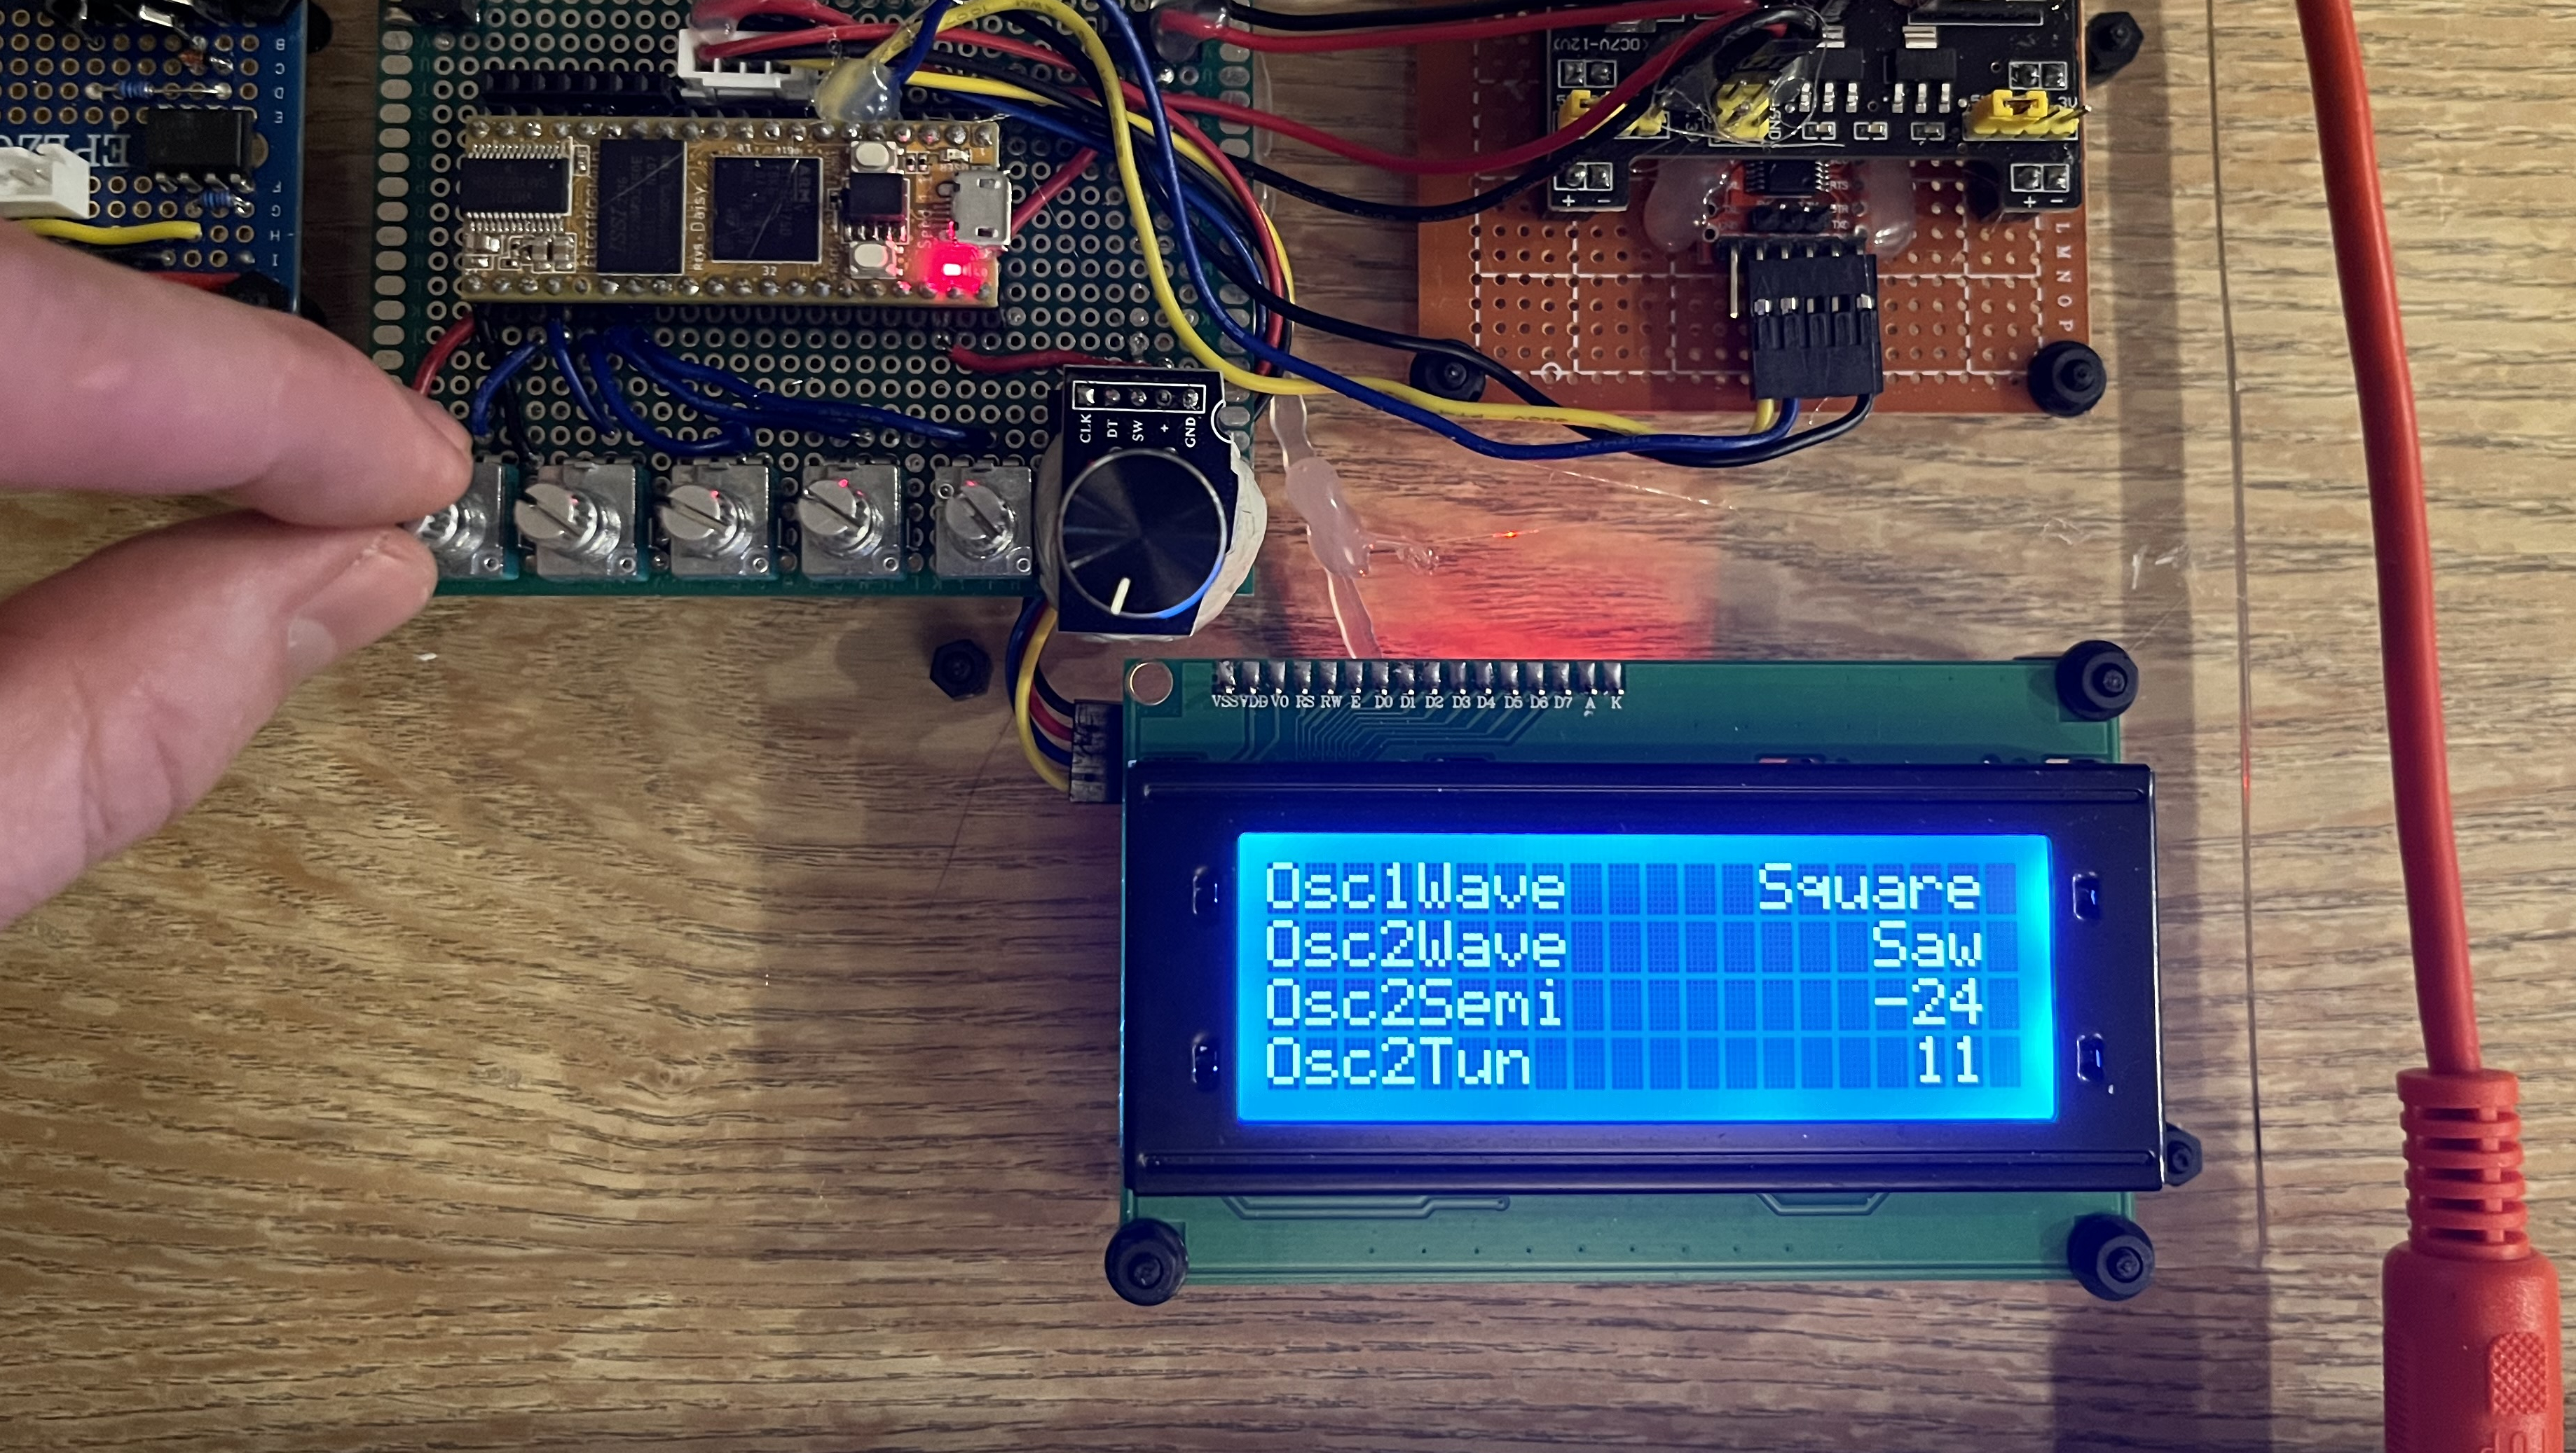
\includegraphics[width=.9\linewidth]{complete_synth_pics/oscillator_context_small}
			\label{fig:sub2}
		\end{subfigure}
		\caption{Navigating the menus with the encoder and using the adaptive potentiometers to mutate system parameters}
		\label{fig:test}
	\end{figure}	

	\subsubsection{High Resolution Digital to Analog Converter (DAC):} 
	\paragraph{The Daisy microcontroller has a built-in high-resolution digital-to-analog converter for playing generated digital audio signals out the speakers}. This DAC is what triggers the audio interrupt callback referred to in the software architecture section. It is responsible for driving the synth to generate samples and convert the samples into an analog signal to play out the speakers. This hardware component is so essential to the software architecture, it's been discussed throughout the paper. Its configuration is quite simple.
	
	\subsubsection{Power, stereo out jack and secondary UART line:}
	\paragraph{The following components are not explicitly tied to the software of the system, but are functionally important to the hardware prototype} The 20x4 LCD screen and the optocoupler on the MIDI input circuit require a 5v power supply, which Daisy does not provide. So simply powering through the Daisy USB port is not an option. Consequently, the system includes a common breadboard power supply. It accepts a barrel jack input providing voltages between 5v and 12v and steps the power down to 5v. This voltage is fed into the VIN pin on Daisy and provides sufficient power for the screen and optocoupler. An 1/8" inch stereo audio jack is connected to the left and right DAC pins on the MCU and outputs audio at line level gain out of the box without the need of an amplifier. Finally, there is a USB to UART converter breakout board connected to a set of RX/TX UART pins on the MCU. This board provides two-way communication between an external computer and the synthesizer via a remote control GUI written in Python.
	
	\subsubsection{Remote Control GUI}
	\paragraph{A remote control GUI app was written to interface with the synth without the hardware interface.} It can be quite useful to those wishing to implement this system without needing to invest time soldering and testing the hardware. The user can spend more time writing new software to extend the system. It works by communicating via USB Serial to tell the synth what parameters to change. The GUI can also save custom patches to a file on the host PC's disk, which can be loaded at will to instantly reconfigure the system. This feature is still in development but is mostly complete. I highly recommend using this tool when adding new audio processing features since it is far less complicated. It's a lot easier to just use the GUI and leave out the hardware peripherals. You would only need to add the MIDI circuit, USB UART breakout and stereo jack to get going.

	\begin{figure}[H]
		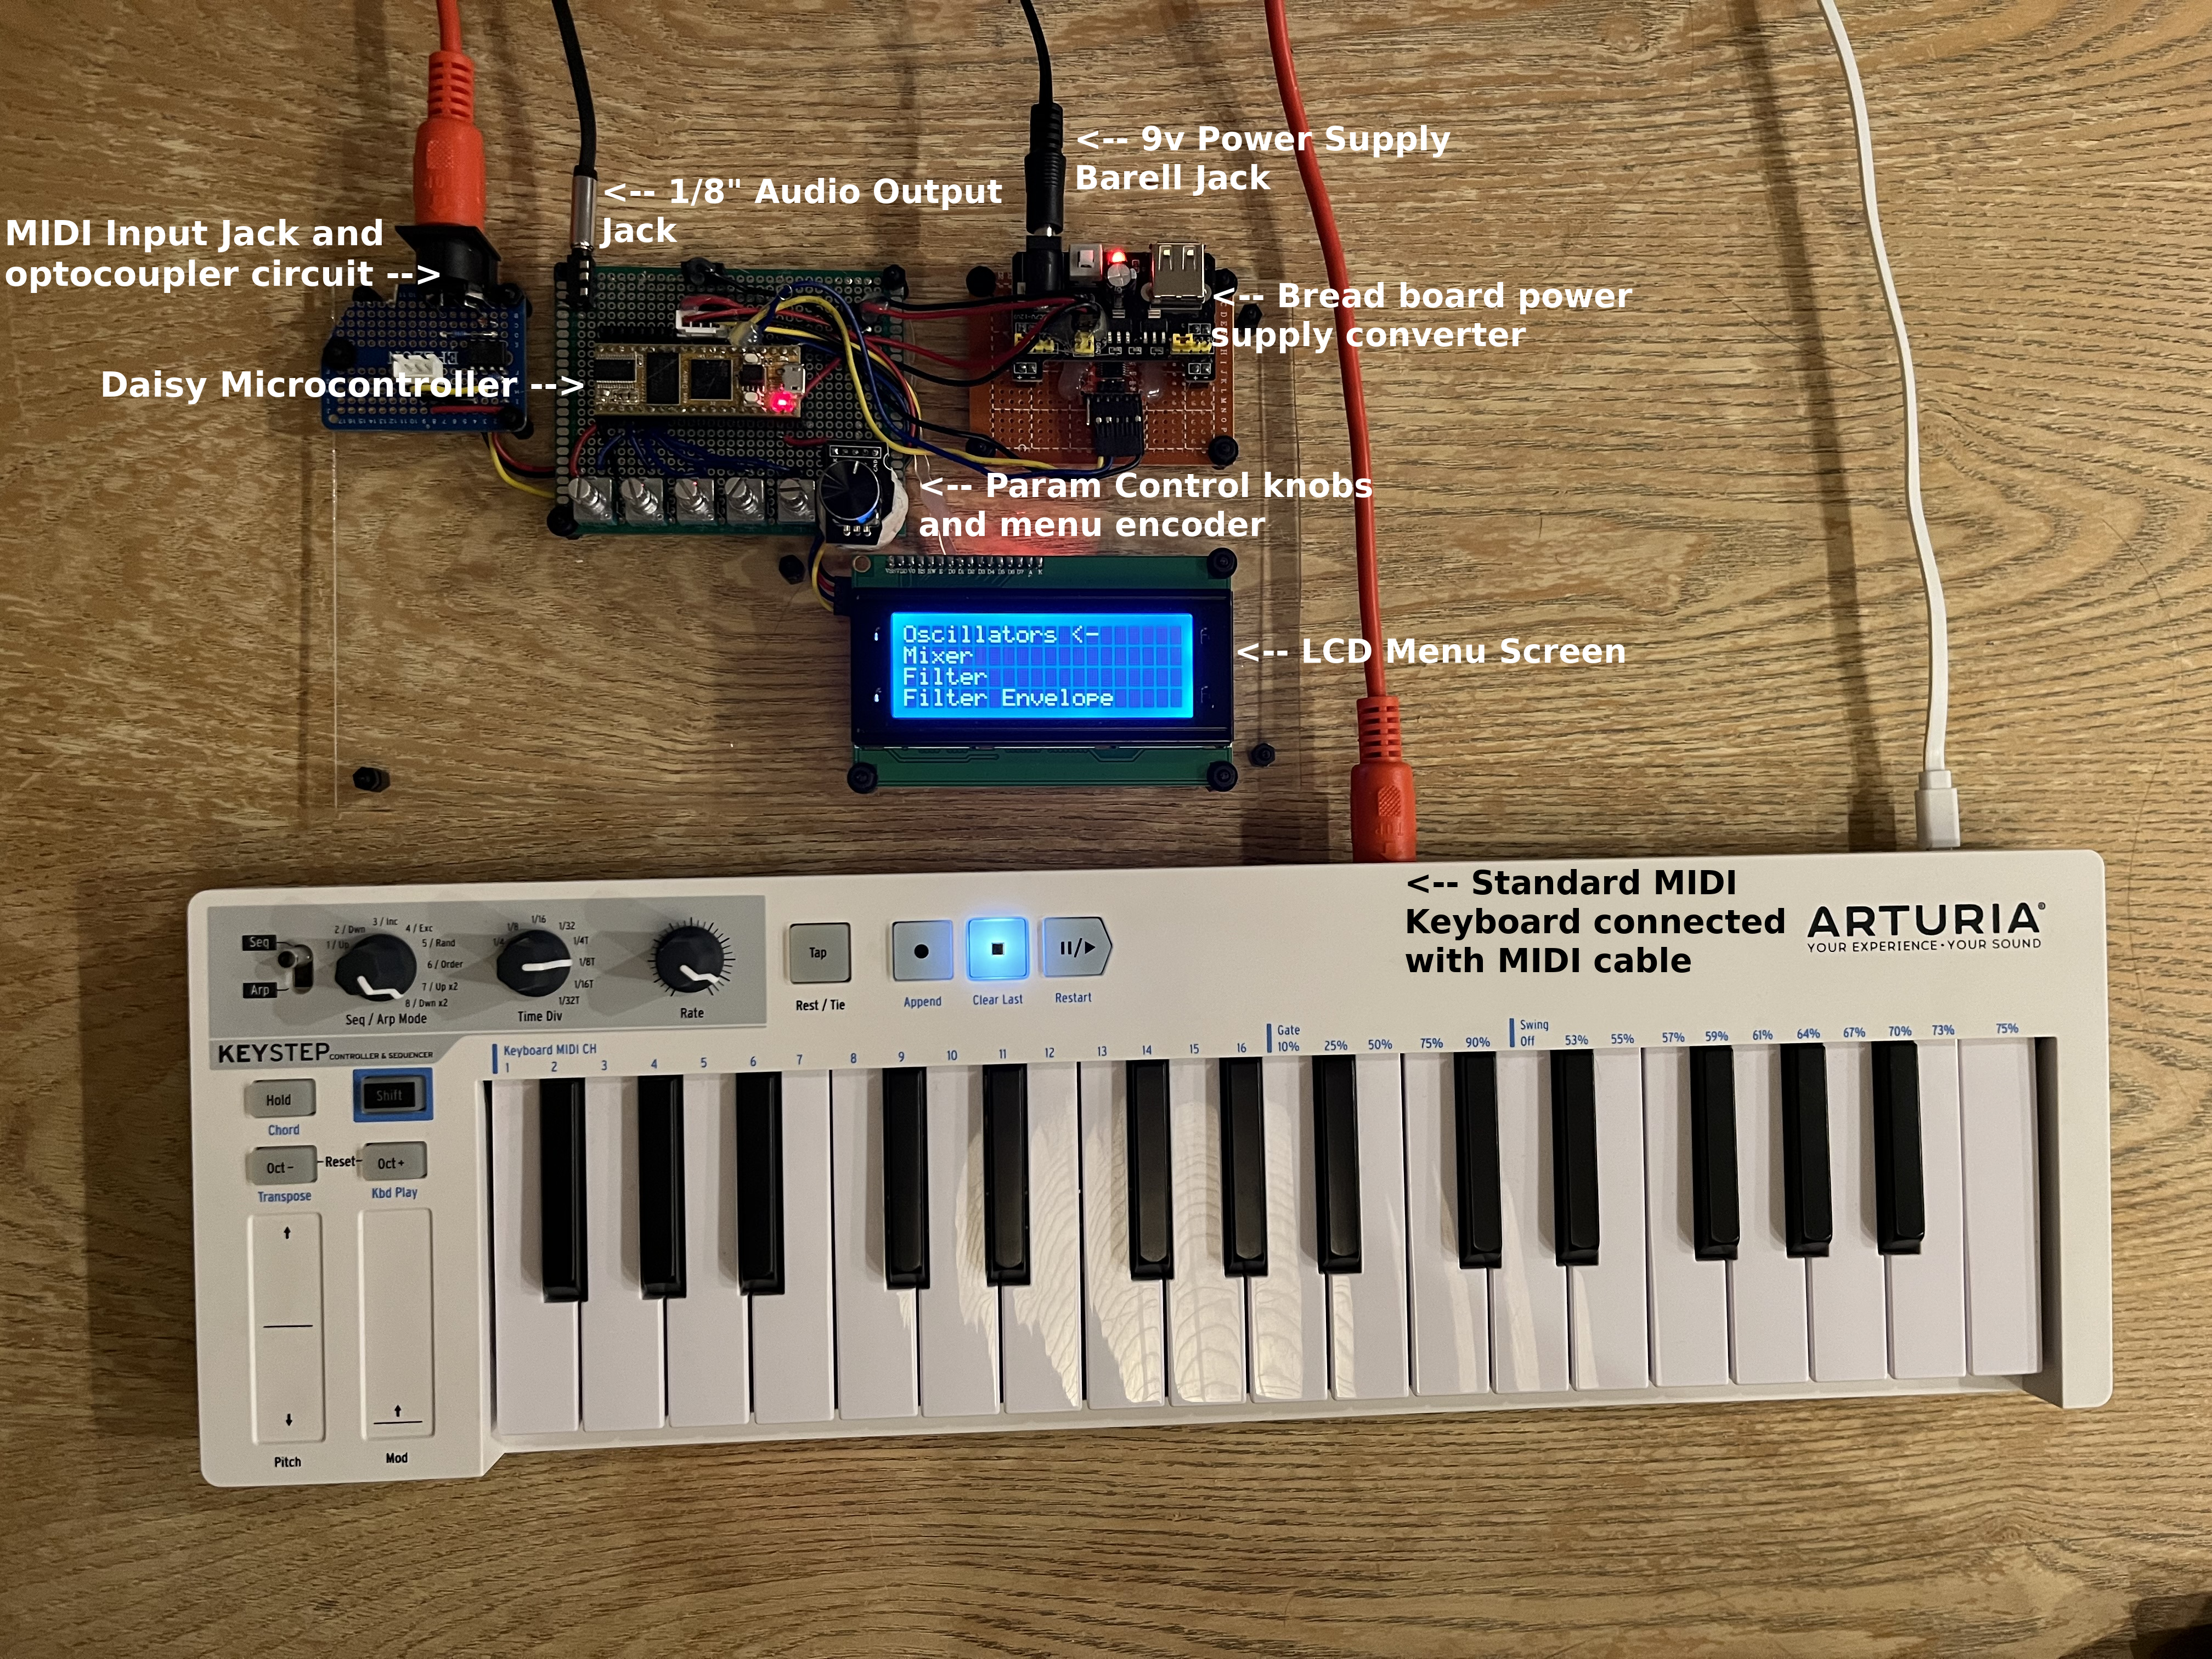
\includegraphics[width=.8\linewidth]{complete_synth_pics/keyboard_and_synth_labeled}
		\caption{The entire synth hardware set up with labels}
		\centering
	\end{figure}

\section{Conclusion}
	\subsection{Successes and completed features} 
	\paragraph{I accomplished the core requirement of my project:} Implement a real-time subtractive synthesizer from scratch on an embedded device. My system uses oscillators to generate tones with pitches based on user input from a generic MIDI keyboard. The tones are combined and processed through an amp envelope to add volume dynamics. The output from the envelope is processed through a filter to carve frequencies out of the audio signal. The final processed audio signal is played out speakers or headphones which can be heard by the user in real-time without interrupts like pops or clicks in the audio.
	
	\subsection{Future Work}
	\paragraph{These features were intended but not strictly necessary for completing the project} There was not enough time to add them within the time frame of the capstone project, but they will be implemented in the future.
	\begin{enumerate}
		\item Flash memory bank for saving patches on the device itself.
		\item Low Frequency Oscillators
		\item Filter Cutoff Envelope
		\item Audio FX Chain
		\item Pitch and mod wheel support for MIDI keyboards
		\item Configuring LFOs and Envelopes to modulate arbitrary signals
	\end{enumerate}
		
	\subsection{Performance Issues and Bottlenecks}
	Overall, there doesn't seem to be much of a bottleneck in the audio pipeline within my project. The synth is never late to deliver audio samples to the DAC, so there are never any audio crackles or pops in the final audio played out the speakers. Most of the time, the CPU is just waiting for the audio and timer callbacks, so there is a lot of processing potential available for adding new features. The only major performance issue that currently persists is the noisiness of the potentiometers. Sometimes I feel like the potentiometers will get super noisy just by looking at them wrong. I plan to fix the noisiness by adding hardware signal filtering to the potentiometers.
	
	\subsection{The Verdict and My Personal Feelings}
	\paragraph{This project was an effective and worthwhile learning experience} A wide breadth of knowledge and wisdom was gained on the process of implementing a complex embedded system. Each module that I added to the system forced me to discover new mathematical tools and concepts. I was pushed to the limits of my understanding, and in the struggle to grasp new concepts, I eventually broke through. These breakthroughs reminded me of the joy that can be experienced in the scientific process. I felt a great sense of empowerment and confidence as previously obscure concepts were demystified. I got to look under the hood and see the inner workings of audio processing. I got a first hand experience of the difficulties of building a complete product from the ground up. The failures I experienced along the way informed me of mistakes to avoid in the future and ways that I can improve my craft as an engineer.

\section{Acknowledgements}
	\paragraph{I would like express my gratitude:}
	\begin{enumerate}
		\item To my wife and children who have been so supportive and patient throughout the whole process. Their love and affection gave me the strength to push through the numerous late nights where I stayed up past 3 writing software and slaving over my soldering work bench.
		\item To my friends and family who showed interest and support in my project and at times offered me advice and encouragement.
		\item To Dr. Frank Jones, my mentor for this project. Until he arrived at UVU, I was constantly begging the school faculty to bring back the Advanced Embedded Systems course to the master's curriculum. Frank's arrival and efforts to revive the embedded systems course is the reason I was able to move beyond blinking LED's on an Arduino and learn the ropes of true embedded systems design.
		\item To Utah Valley University and its staff. I've studied at this institution since 2014 and will have graduated twice from it come next week. I got my undergraduate degree in Commercial Music and discovered engineering in the process. I continued to take classes until I fulfilled requirements to start the Master's of Computer Science program. Now I am at the end of my graduate program and I have already enjoyed the benefits of a lucrative and fulfilling career. I owe so much to UVU for their openness to all who wish to learn and their dedication to educating and uplifting its students.
	\end{enumerate}

	\paragraph{I would also like to give credit to all the silent hero's of the computer science and open source community} We stand on the shoulders of giants. The things we accomplish now are only possible because of the charitable efforts of other engineers. The free software tools, compilers, blog posts, instructional videos and documentation are indispensable assets that have made the joys of computers accessible to nearly every human being in the world. The development of low cost hardware, high level programming languages and free learning resources made it possible for me to discover my passion for engineering. It gave me the courage to leave my career path as a profession musician that was leaving me jaded to music and creatively unfulfilled. Now, my preferred choice of artistic expression is through the medium of engineering. I owe so much to the millions of people who contribute to the open source world making computer science accessible to everyone.

\bibliographystyle{ACM-Reference-Format}
\bibliography{sources.bib}

\pagebreak


%%
%% If your work has an appendix, this is the place to put it.
\appendix

\section{User's Manual}
\subsection{Getting started}
\textbf{To start making some noise, you will need}
\begin{itemize}
	\item A nine volt power supply
	\item A keyboard with a MIDI output jack
	\item A standard MIDI cable
	\item A set of headphones or speakers
\end{itemize}
\paragraph{Start by connecting the power supply to the synth} Connect your headphones or speakers to the 1/8" stereo output. Connect the MIDI cable to the output jack of your keyboard and the input jack of the synth. Press the toggle switch next to the barrel jack on the synth the power up the system. The screen will illuminate and display the main menu. On boot, the synth will already be configured with a default patch. You should now be able to hear music play out the speakers by pressing keys on the keyboard. If you cannot hear anything, the master volume may need to be adjusted. The knob next to the rotary encoder is the master volume and is always mapped to control master volume in any menu context. Turning it clock wise increase the master volume and you should now be able to hear the synth playing a simple sin wave.

\subsection{Navigating the menu}
\paragraph{The menu system is navigated using the rotary encoder} Turn the encoder to scroll the menu and view the available menu contexts. An arrow icon will point to the submenu that will be selected when you press the encoder button down. When you find a menu you wish to configure, highlight it with the arrow icon and press down on the encoder. The menu will clear and render parameters of the submenu. At this point, the potentiometers are active and mapped to alter the parameters of this menu. The parameters listed on screen from top to bottom map to the first four potentiometers from left to right. Move the leftmost potentiometer will adjust to the top parameter in the screen and so on. To return to the main menu, turn the rotary encoder any direction.

\subsection{Using the multipurpose knobs}
\paragraph{The first four potentiometers from left to right map to the parameters on screen from top to bottom.} Depending on the selected menu, the values read from the knobs and displayed on screen will be different. Sometimes, the knob values may represent a discrete number in a numeric range, or they may just represent a specific type or setting like "sawtooth" for oscillator waveform. Moving a knob will not affect any change in the parameters unless the read value describes a new setting inside the mapped range. Since the knobs are multipurpose, you may need to move the knob a bit in one direction before seeing the change take affect. This is intentional so that you do not accidentally erase any existing settings you may have had because the knobs were moved to a new position while in a separate context. While in a menu context, only the parameters of that menu will be mutable. All other parameters will remain unchanged until you navigate back to the submenu that controls them. Once you are done changing parameters, move the menu context knob to return to the main menu and all parameters will be in an immutable state.

\subsection{Configuring oscillators}
\paragraph{To configure the oscillator waveforms, turn the menu encoder until the Oscillators submenu is highlighted by the arrow icon.} Press down the menu encoder to select the oscillator menu. The screen will reprint to display the current configuration of the oscillators:\\
	\begin{enumerate}
		\item Osc1Wave - Sin, Saw, Triangle, Square and Noise
		\item Osc2Wave - Same as Osc1Wave
		\item Osc2Semi - Semitone offset added to oscillator 2 pitch. Range from -24 to +24 (two octave below and above)
		\item Osc2Tune - Hertz offset added to oscillator 2. Much smaller than semitones, used to for more subtle tuning and detuning.
	\end{enumerate}

\paragraph{To change the waveforms of the oscillators, rotate knobs 1 and 2 until the waveforms listed on the LCD screen begin to change.} If you are not sure whether you need to rotate clockwise or counter-clockwise, it may be a good idea to rotate all the way counter-clockwise until the knob is at its minimum value. Then you can start turning the knob until you select your desired waveform. After some practice and familiarizing yourself with the order of the waveforms, you will gain an intuition for which way you should turn the knobs to configure the waveforms more quickly. This same technique applies to all other parameters. The Osc2Semi parameters represents how many note values you are pitching up or down the second oscillator. You can pitch it down two full octaves, up to octaves or any number of semitones in between. Osc2Tune will apply a more granular level of pitch control in hertz. This allows you to alter the pitch to fit in between semitones to make the notes sharp or flat in relation to conventional keyboard tunings.

\subsection{Configuring the amp envelope}
\paragraph{To configure the amp envelope, turn the menu encoder until the Amp Envelope submenu is highlighted by the arrow icon.} Press down on the encoder to select the Amp Envelope menu. The screen will reprint to display the current envelope configuration:\\
	\begin{enumerate}
		\item Attack - How long it takes to reach maximum gain on the envelope in milliseconds (5-5000ms)
		\item Decay - How long it takes to reach the sustain gain on the envelope in milliseconds (5-5000ms)
		\item Sustain - The value of the sustain gain (0-1.0). The lower the value, the more quiet the voices will be during sustain.
		\item Release - How long it takes for the gain to diminish back to 0 after releasing a note (5-5000ms).
	\end{enumerate}

\paragraph{The envelope configuration is easier to intuitively configure with the adaptive knobs}. Since the knobs are mapped to a range with many more values, moving the knobs will change the values almost immediately on screen. If you set a long attack value and press down on the keyboard, you will notice that the notes take much longer to reach max gain and will appear to swell in volume. The same observations can be made by setting longer sustain and release values. As an exercise, you can try setting up the envelope to mimic the dynamics of a guitar: Set the attack to 10ms, sustain and release to 500ms and decay to 0.5. The synth will now play notes with a percussive affect like plucking strings. The voice will reach full volume very quickly and then fade away slowly over time.

\subsection{Filters and Mixer} 
\paragraph{These menus contain some usable parameters but some parameters remain inactive as they require additional features.} To change the mix between the two oscillators within the voices, select the Mixer menu. Osc1 Lvl and Osc2 Lvl contain the gain value for each respective oscillator ranging from 0-1.0. To get a 50/50 mix of the two oscillators, set each parameter to 0.5. You can play with the mix by making one oscillator louder than the other. The configure the filter, select the the Filter menu. The cutoff parameter will affect what frequency the filter will begin to attenuate a the frequency spectrum and has a range from (100hz to 20000hz). If filter type is set to low pass, setting the frequency to 20000hz will affectively let all frequencies pass through resulting in the signal remaining unaffected. Setting the cuttoff to 1000hz will cut out most of the high frequency harmonics resulting in a much more mellow sound. Altering the resonance parameter will creating a gain boosting affect around the cutoff point on the filter with values ranging between 0-8.0. Setting a very high resonance factor will cause a lot of boosting around the cutoff point. It may not be immediately obvious, but "sweeping" the cutoff frequency by turning the knob as you play a note will demonstrating the boosting effect around the cutoff point. A more audible whirring or swishing affect can be heard (a classic sound effect often used with synthesizers).

\subsection{Using the Remote Control GUI} To use the GUI app, you will need a USB Mini cable. Connect the USB Mini jack to the serial interface board located directly under the power supply board on the synth and your host PC. The source code is included in the synth repo as a submodule. By running \textit{git submodule update --init --recursive} within the main repo, the submodule \textit{serial\_control\_interface} will be cloned. \textit{cd} into this directory. It is written in python and utilizes the pyserial library and PySimpleGUI.

To get started, create a python virtual environment and install the required libraries by running \textit{pip install -r requirements.txt}. The program can now be run with the command \textit{python main.py <serial device descriptor>}. On a standard linux ubuntu distribution, the device descriptor will appear as /dev/ttyUSB0. You may need to add your user to the \textit{dialout} group to have permissions to access serial devices.

After you run this command, the GUI window will pop up with several tabs. The interface should be familiar with all the same available parameters available to change as in the menu screen. Moving the sliders or selecting a radio button will tell the GUI backend to transmit a command through the serial wire with encoded parameter data.

\section{Related Works}
\begin{description}
	\item[Designing Sound by Andy Farnell] A practical guide to digital audio synthesis. Describes the common structures of DSP using a visual programming language called PureData. Used as primer for understanding modules implemented in this project.
	\item[Think DSP: Digital Signal Processing in python by Allen Downey] DSP examples written in python. Referenced for generating oscillator functions and understanding concepts of filtering.
	\item[Embedded Systems Architecture by Daniele LaCamera] Comprehensive textbook on embedded systems. Heavily referenced for hardware configuration and firmware design.
	\item[Audio effects: Theory, implementation, and application by Joshua Reiss and Andrew McPherson] References in implementations of audio fx (filters, reverb, delay, phaser etc). Referenced for planned but yet unimplemented audio fx chain.
	\item[Subtractive synthesis: The synthesizer academy by Scott Rise] Blog post on subtractive synthesis. Referenced as industry definition of subtractive synthesis and its applications.
	\item[Learning synthesis: Oscillators by Eldar Tagi] Blog post explaining different types of oscillators, waveforms and their implementations in analog and digital domain. Referenced for study of the history of synthesis, definition of frequency modulation and the functions of oscillators.
	\item[microKorg by Korg] A compact polyphonic analog synthesizer. An industry standard instrument used as a reference when defining the requirements of the project.
	\item[What is a LFO and how to use it by Vanesa Paris] A blog post explaining the mechanics and applications of Low Frequency Oscillators. A reference for the requirements of the unimplemented LFO module.
	\item[Midi for the Arduino - Build a Midi Input Circuit] A blog post explaining how to implement an optocoupler protected midi input circuit to an Arduino. This circuit was implemented in its entirety and adapted to work with the Daisy platform.
	\item[Materials for Linear Algebra: Linear Filters by Joshua Holden] A free Duke University text book referenced extensively for understanding discrete time signal filtering with difference equation.
	\item[Introduction to Digital Filters with Audio Applications by Julius Smith] A free Stanford University textbook on Digital Filters. Referenced heavily for learning about transfer functions, bilinear transform and second order difference equation.
	\item[Introduction to Computer Music by Jeffrey Hass] Indiana University text book covering analog and digital synthesis concepts, filters, envelopes, etc. Very comprehensive and referenced for research on envelopes, filters and oscillators.
	\item[libDaisy by Electro-Smith] Open source hardware abstraction layer library for the Daisy ecosystem. Heavily used in implementation for settings up DAC/Timer interrupts, potentiometer ADCs, digital encoder reading and I2C bus setup.
	\item[Welsh's synthesizer cookbook by Fred Welsh] A "cookbook" for setting up any generic synthesizer to emulate sounds like pianos, violins, banjo, guitar etc. Referenced for researching concepts of subtractive synthesis.
	\item[The MIDI Manual by David Miles Huber] A comprehensive textbook covering the MIDI protocol. Referenced for explanations of how data is packed into MIDI messages.
\end{description}

\end{document}
\endinput
%%
%% End of file `sample-manuscript.tex'.
